\documentclass[a4paper]{article}

%\setlength{\parskip}{0.5\baselineskip}

\usepackage{geometry}
\geometry{left = 2.54 cm, right = 2.54 cm, top = 2.54 cm, bottom = 2.54 cm}

\usepackage{setspace}
\renewcommand{\baselinestretch}{1.0}
\usepackage{indentfirst}
\setlength{\parindent}{2em}

%\usepackage{fontspec}
%\setmainfont{Times New Roman}

\usepackage[]{cprotect}

\usepackage{hyperref}
\hypersetup{
  colorlinks=true,
  linkcolor=blue,
  filecolor=magenta,
  urlcolor=cyan,
}

\usepackage{ulem}
\usepackage{graphicx}
%\usepackage{wrapfig}
\usepackage{enumitem}
\usepackage{xcolor}
\usepackage{subcaption}
\usepackage{float}
\usepackage{amsmath, amssymb, amsthm}
\usepackage{booktabs}

\usepackage{listings} % Required for insertion of code

\lstdefinestyle{lzx}{
    % basicstyle = \small\ttfamily\fontfamily{cmr}\selectfont,
    basicstyle = \ttfamily \footnotesize,
    keywordstyle = \color{purple}\bfseries,
    % commentstyle = \color{green}\itshape,
    commentstyle = \color[RGB]{116, 153, 62}\ttfamily,
    stringstyle = \ttfamily,
    %
    tabsize = 2,
    showspaces = false,
    numberstyle = \ttfamily\color[RGB]{0,96,96},
    showstringspaces = false,
    captionpos = t,
    %
    showlines = true,
    emptylines = *2, % 2 for python, 1 for other language
    numbers = left,
    xleftmargin = 5mm,
    numbersep = 5pt,
    linewidth = \linewidth,
    % backgroundcolor=\color{red},
    frame = single,
    frameround = tttt,
    framexleftmargin = 7mm,
    %
    breaklines = true,
    postbreak = \mbox{\textcolor{red}{\( \hookrightarrow \)}\space},
}

\lstset{
    style = lzx, %
}

%\pagestyle{empty} % Not showing page number

\begin{document}
\renewcommand{\thesection}{\Roman{section}}
\renewcommand{\thesubsection}{\Alph{subsection}}
\renewcommand{\thesubsubsection}{\thesubsection.\arabic{subsubsection}}
\renewcommand{\d}{\: \mathrm{d}}
\newcommand{\e}{\mathrm{e}}

\begin{center}
  \textbf{\Large VE373 Recitation Class}\\[1em]
  \textbf{\large Week 3} \\[1em]
  2022.05.28 \\[1em]
\end{center}

\section*{L4 --- Timers and IO}
  \begin{enumerate}[label = \arabic*.]
    \item \textbf{GPI/O Ports}
      \par Each port has 4 associated registers for its operation:
      \begin{itemize}[leftmargin = 1cm]
        \item \verb|TRISx| register: Data Direction register, or Tri-State Control register
          \begin{itemize}[leftmargin = 1cm]
            \item \verb|1| for input
            \item \verb|0| for output
            \item all port I/O pins are defined as inputs after a device Reset. Certain I/O pins are shared with analog peripherals and default to analog inputs after a device Reset.
          \end{itemize}
        \item \verb|LATx| register: output latch
          \begin{itemize}[leftmargin = 1cm]
            \item used to write date to the port I/O pins. The \verb|LATx| Latch register holds the data written to either
              the \verb|LATx| or \verb|PORTx| registers.
            \item reading the LATx Latch register reads the last value written to the corresponding PORT or Latch register.
          \end{itemize}
        \item \verb|PORTx| register: reads the levels on the pins of the device
          \begin{itemize}[leftmargin = 1cm]
            \item used to read the current state of the signal applied to the port I/O pins
            \item writing to a \verb|PORTx| register performs a write to the port's latch, \verb|LATx| register, latching the data to the port's I/O pins
          \end{itemize}
        \item \verb|ODCx| register: Open-drain control
          \begin{quotation}
            \par Pins are configured as digital outputs by setting the corresponding \verb|TRIS| register bits = 0. When configured as digital outputs, these pins are CMOS drivers or can be configured as open-drain outputs by setting the corresponding bits in the Open-Drain Configuration (\verb|ODCx|) register.
            \par The open-drain feature allows generation of outputs higher than \( V_{DD} \) (e.g., 5V) on any desired 5V tolerant pins by using external pull-up resistors. The maximum open-drain voltage allowed is the same as the maximum \( V_{IH} \) specification.
          \end{quotation}
      \end{itemize}

    \item \cprotect\textbf{\verb|CLR|, \verb|SET| And \verb|INV| Registers}
      \par Provide fast atomic bit manipulations, perform operation in hardware atomically.
      \par Reading SET, CLR and INV registers returns undefined
      values.
      \par E.g. \verb|T2CONSET = 0x8000| in homework 1.
  \end{enumerate}

\section*{L5 --- Interrupts}
  \begin{enumerate}[label = \arabic*.]
    \item \textbf{Detect events}
      \par Dealing with asynchronous events:
      \begin{itemize}[leftmargin = 1cm]
        \item Exceptions caused by program execution
        \item Peripheral needs attention or has completed a requested action
        \item Application makes a system call
      \end{itemize}


    \item \textbf{Software polling}
      \begin{itemize}[leftmargin = 1cm]
        \item We can repeatedly poll the application for peripherals.
        \item When an event occurs, detect this via a poll and take action
        \item Common in small or low-performance real-time embedded systems
          \begin{itemize}[leftmargin = 1cm]
            \item Predictable timing
            \item Low hardware cost
          \end{itemize}
        \item In other systems, wastes CPU time
          \begin{itemize}[leftmargin = 1cm]
            \item Affect processor's responsiveness and efficiency
          \end{itemize}
      \end{itemize}
      \begin{lstlisting}[language=c]
/* Timer control */
T2CON = 0x0;       // Stop Timer2 and clear control register
                   // prescale 1:1, internal clock source
TMR2 = 0x0;        // Clear Timer
PR2 = 0xFFFF;
T2CONSET = 0x8000; //Start Timer2

/* polling */
while (TMR2 != 1000);

/* move on */
...
      \end{lstlisting}
    \item \textbf{Interrupt}
      \begin{itemize}[leftmargin = 1cm]
        \item Let the application for peripheral notify us automatically.
        \item Take action (respond to the event) when such a notification occurs (or shortly later).
      \end{itemize}

      \par When a special event or error occurs
      \begin{itemize}[leftmargin = 1cm]
        \item I/O controller interrupts CPU -- by a call from the I/O hardware
        \item CPU stops executing the current program
        \item CPU goes to run an \textbf{interrupt handler} (a special piece of program) or \textbf{interrupt service routine} (ISR)
        \item After finish executing the ISR, CPU returns back to the interrupted program and resume
        \item Not synchronized to instruction execution, may happen between any two instructions
      \end{itemize}
    \item \textbf{Typical Types of Interrupts}
      \begin{itemize}[leftmargin = 1cm]
        \item Internal (exception)
          \begin{itemize}[leftmargin = 1cm]
            \item By CPU errors
            \item By bad instructions
          \end{itemize}
        \item External (interrupt)
          \begin{itemize}[leftmargin = 1cm]
            \item External I/O device
            \item Timer
            \item Reset
            \item System failure
          \end{itemize}
      \end{itemize}
      \par Interrupt comes as a high-level signal or a rising edge depending on processors

    \item \textbf{SFRs for Interrupt}
      \begin{itemize}[leftmargin = 1cm]
        \item \verb|INTCON| -- Interrupt Control Register
        \item \verb|INTSTAT| -- Interrupt Status Register
        \item \verb|TPTMR| -- Temporal Proximity Timer Register
        \item \verb|IFSx| -- Interrupt Flag Status Registers
        \item \verb|IECx| -- Interrupt Enable Control Registers
        \item \verb|IPCx| -- Interrupt Priority Control Registers
      \end{itemize}

    \item \textbf{Interrupt Control}
      \begin{enumerate}[label = \arabic*.]
        \item Enable interrupt globally
        \item Config \verb|INTCON| to select multi vector mode.
        \item Enable individual interrupt, set priority
        \item When interrupt event happens, flag is set regardless of the enable bit
        \item If enabled, interrupt service routine (ISR)
        \item In ISR, service interrupt, clear interrupt flag (for most interrupt requests)
        \item Main program resumes
      \end{enumerate}

    \item \textbf{Enable/disable all interrupt sources globally}
      \begin{itemize}[leftmargin = 1cm]
        \item \verb|asm("ei"); // inline MIPS32 assembly|
        \item \verb|asm("di");|
        \item Corresponding to enable/disable IE bit (\verb|STATUS<0>|)
        \item Must be enabled before individual interrupt can be used
      \end{itemize}

    \item \textbf{Operation Mode}
      \begin{itemize}[leftmargin = 1cm]
        \item Controlled by \verb|MVEC| bit in \verb|INTCON|
        \item \textbf{Single vector mode:}
          \begin{itemize}[leftmargin = 1cm]
            \item All interrupt requests will be serviced at one vector address (default upon reset)
            \item One location for all different interrupts
            \item have to determine what exception/interrupt has just happened, by checking status registers
            \item \verb|if...else...| structure
          \end{itemize}
        \item \textbf{Multi vector mode:} Interrupt requests will be serviced at the calculated vector address
          \begin{itemize}[leftmargin = 1cm]
            \item One location for one (or a small number of) interrupt
            \item Take actions or handle interrupts directly
          \end{itemize}
      \end{itemize}

    \item \textbf{Interrupt Vector Table}
      \begin{figure}[H]
        \centering
        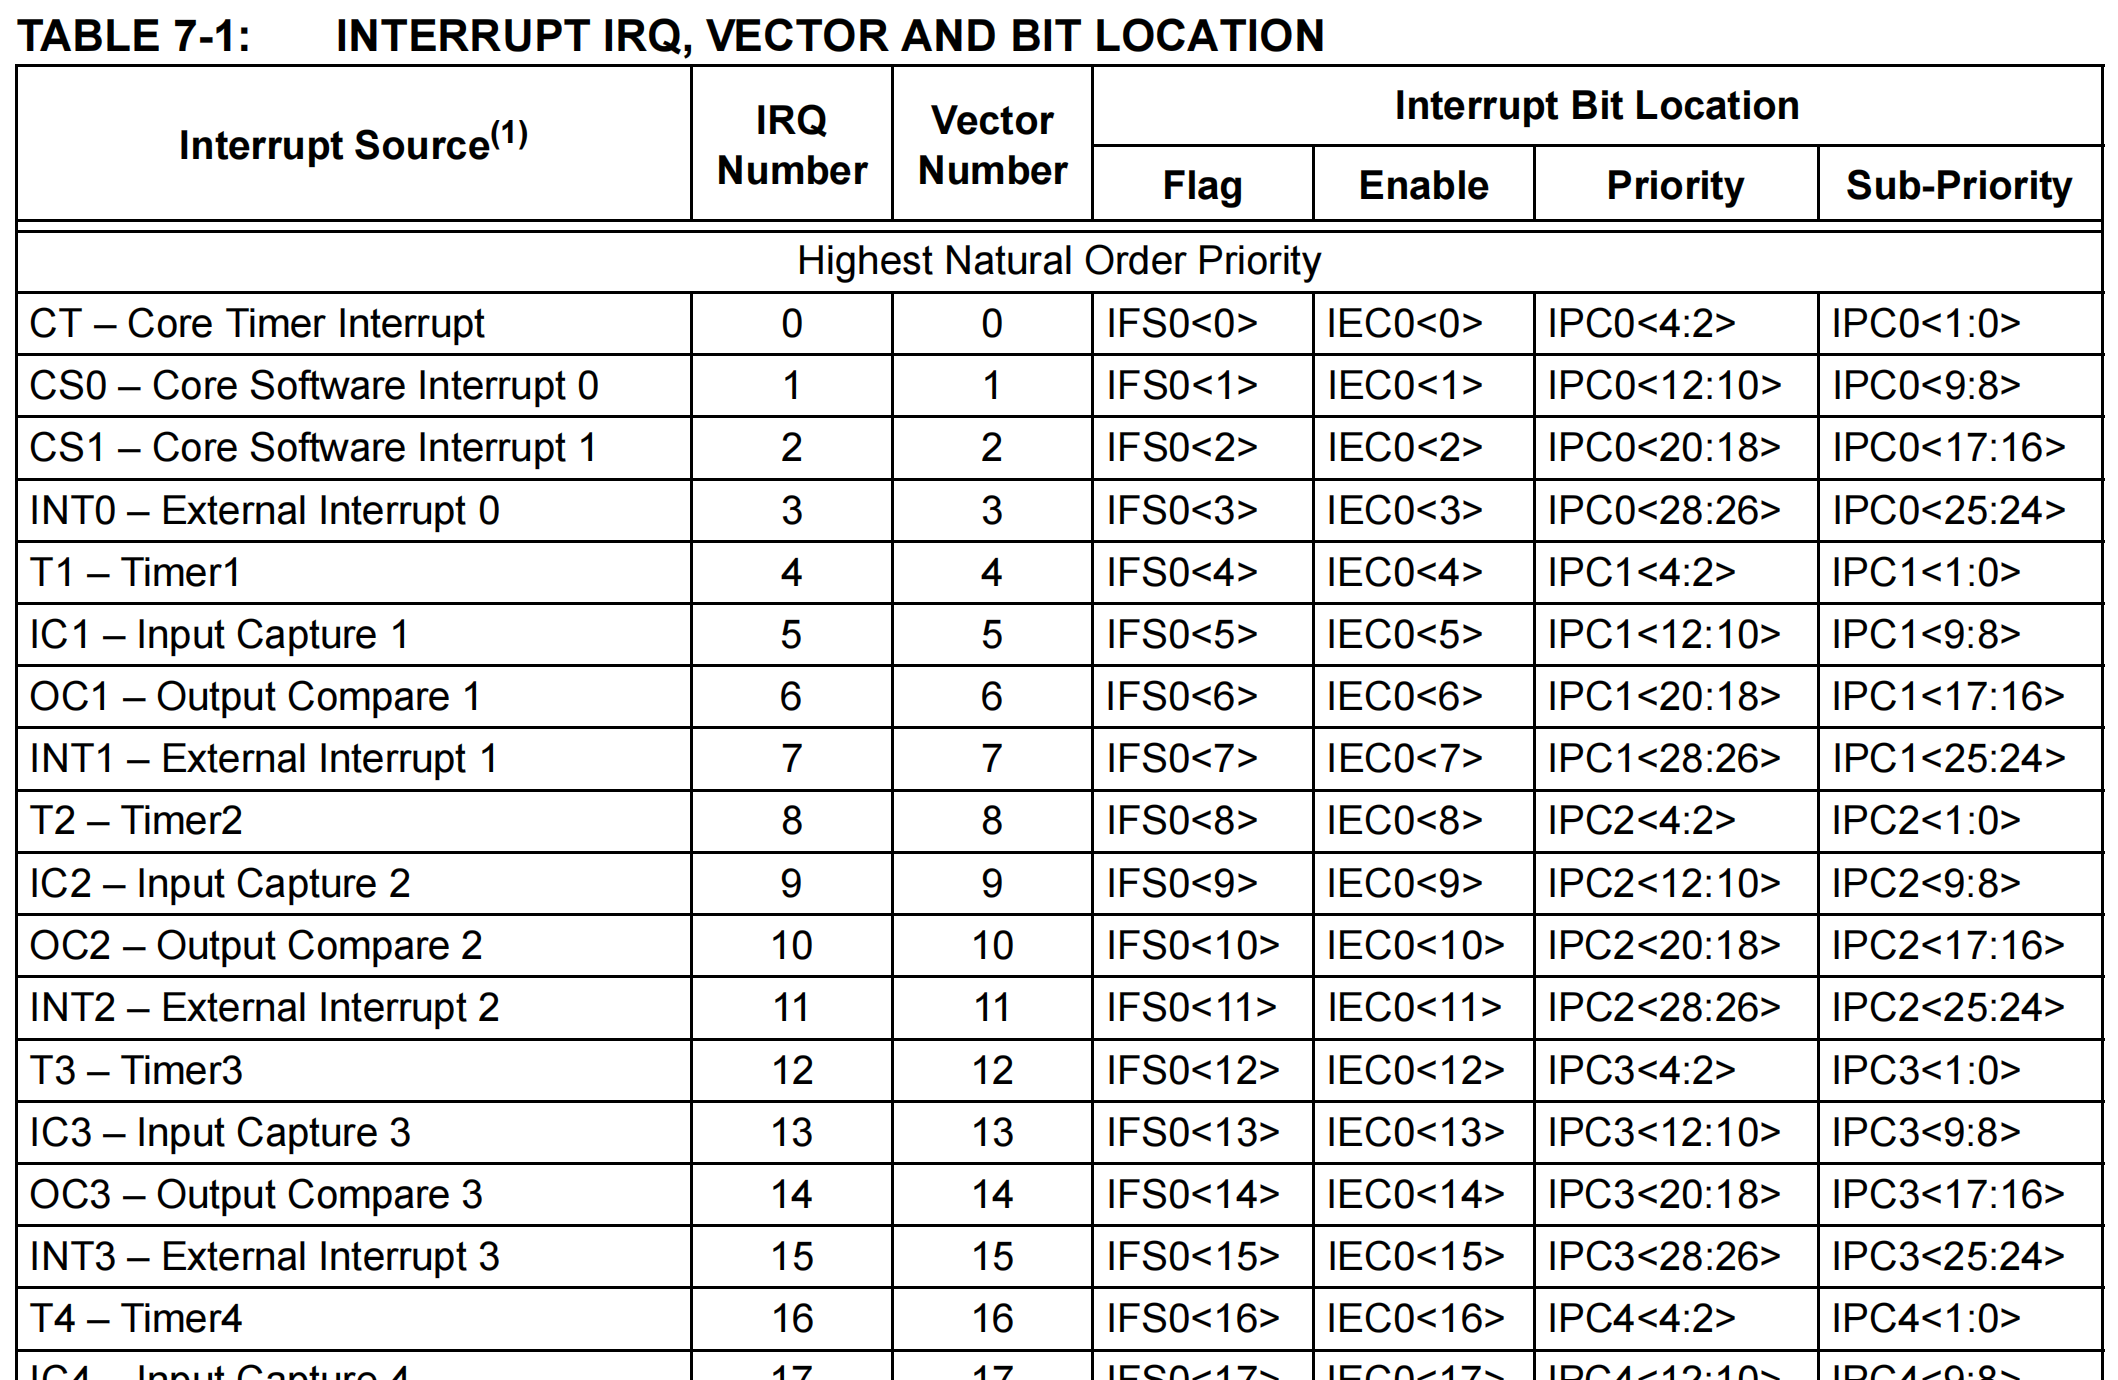
\includegraphics[width=0.9\linewidth]{Interrupt_table.png}
        \label{fig:Interrupt_table.png}
      \end{figure}

    \item \textbf{ISR -- Interrupt Service Routine}
      \par Discussed in the next week's RC\@.

  \end{enumerate}

\section*{Tips for Homework}
  \begin{quotation}
    Define a new 32-bit SFR named \verb|MCUCON| as a C structure. The SFR contains four fields:
    \begin{itemize}[leftmargin = 1cm]
      \item \verb|ON|: in \verb|MCUCON[31]|
      \item \verb|MODE|: in \verb|MCUCON[24:22]|
      \item \verb|STATUS|: in \verb|MCUCON[15:8]|
      \item \verb|IPL|: in \verb|MCUCON[7:6]|
    \end{itemize}
  \end{quotation}
  \par You can refer to the header file of the PIC32 board we use. You have two ways to find it:
  \begin{enumerate}[label = \arabic*.]
    \item Access it on \href{https://github.com/jasonkajita/pic32-part-support/blob/master/include/proc/p32mx795f512l.h}{github}.
    \item You can create a test.c file, include header file \verb|p32xxxx.h|, and write a SFR in \verb|main()| (e.g. \verb|T1CON|). Then by holding ctrl and clicking on it, you can navigate to its definition through the built-in function of IDE\@. You may want to do that in future labs.
  \end{enumerate}
  \par The header file defines \verb|T1CON| as shown below:
  \begin{lstlisting}[language=c]
#define T1CON T1CON
extern volatile unsigned int   T1CON __attribute__((section("sfrs")));
typedef union {
  struct {
    unsigned :1;
    unsigned TCS:1;
    unsigned TSYNC:1;
    unsigned :1;
    unsigned TCKPS:2;
    unsigned :1;
    unsigned TGATE:1;
    unsigned :3;
    unsigned TWIP:1;
    unsigned TWDIS:1;
    unsigned SIDL:1;
    unsigned :1;
    unsigned ON:1;
  };
  struct {
    unsigned :4;
    unsigned TCKPS0:1;
    unsigned TCKPS1:1;
  };
  struct {
    unsigned :13;
    unsigned TSIDL:1;
    unsigned :1;
    unsigned TON:1;
  };
  struct {
    unsigned w:32;
  };
} __T1CONbits_t;
extern volatile __T1CONbits_t T1CONbits __asm__ ("T1CON") __attribute__((section("sfrs")));
extern volatile unsigned int        T1CONCLR __attribute__((section("sfrs")));
extern volatile unsigned int        T1CONSET __attribute__((section("sfrs")));
extern volatile unsigned int        T1CONINV __attribute__((section("sfrs")));
  \end{lstlisting}
  \par You only need to define the union as shown above.


\end{document}